
\begin{definition} \label{definition:order_k_Bspline}
Let $t= \left\{ t_i \right\}$ denote a non-decreasing sequence. The $i^{th}$ B-spline of order $k$ which corresponds to the knot sequence $t$ is defined by 
\begin{equation} \label{eq:bspline_definition}
B_{i,k,t}\left(x\right) = \left(t_{i+k}-t_i\right)\left[t_i,\dots,t_{i+k}\right]\left(\cdot -x\right)_+^{k-1}
\end{equation}
\end{definition}

The placeholder notation, $\left(\cdot - x\right)_+^{k-1}$, is used to indicate that the $k^{th}$ divided difference of the function $g\left(t \right) = \left(t-x\right)^{k-1}_+$ is obtained by fixing $x$ and applying the divided difference to $g\left(t \right)$ as a function of $t$ alone. Henceforth, we will write $B_i$ rather than $B_{i,k,t}$ when the spline order and knot sequence can be inferred from surrounding context.

\subsection{Properties of B-splines}

\begin{enumerate} \label{eq:BS_properties}
\item \label{eq:BS_property_1} $B_i\left(x\right)$ has isolated support:
\[
B_i\left(x\right) = 0, \quad x \not \in \left[t_{i},t_{i+k}\right]
\]
To see this, note that if $x \not \in \left[t_{i},t_{i+k}\right]$, then $g\left(t \right) = \left(t-x\right)^{k-1}_+$ is a polynomial of degree $< k$ on $\left[t_{i},t_{i+k}\right]$, thus by \ref{dd_properties} \ref{eq:dd_property_5},
\[
\left[t_{i},\dots,t_{i+k}\right]g = 0.
\]
As a result, for a set of B-splines of order $k$ corresponding to the knot sequence $t$, only $k$ of them are nonzero on $\left[t_{j},t_{j+k}\right]$: $B_{j-k+1},B_{j-k+2},\dots,B_{j}$.
\item \label{eq:BS_property_2} The $i^{th}$ B-spline of order is defined as the $k^{th}$ divided difference of $\left(\cdot - x\right)_+^{k-1}$ times a normalization factor: $\left(t_{i+k}-t_i\right)$. This normalization, using \ref{dd_properties} \ref{eq:dd_property_8}, allows us to write 
\begin{equation} \label{eq:BS_norm_rr}
B_i\left(x\right)=\left[t_{i+1},\dots,t_{i+k} \right]\left(\cdot - x\right)_+^{k-1} - \left[t_{i},\dots,t_{i+k-1} \right]\left(\cdot - x\right)_+^{k-1}
\end{equation}
For $x \in \left(t_{j},t_{j+1}\right)$, by \ref{dd_properties} \ref{eq:dd_property_1},
\begin{align}
\sum_{i} B_i\left(x\right) &=  \sum_{i=j+1-k}^{j} B_i\left(x\right) \nonumber\\
&= \sum_{i=j+1-k}^{j} \left[t_{i+1},\dots,t_{i+k} \right] \left(\cdot - x\right)_+^{k-1} - \sum_{i=j+1-k}^{j} \left[t_{i},\dots,t_{i+k-1} \right] \left(\cdot - x\right)_+^{k-1} \nonumber \\
&= \left[t_{j+1},\dots,t_{j+k} \right] \left(\cdot - x\right)_+^{k-1} - \left[t_{j+1-k},\dots,t_{j} \right] \left(\cdot - x\right)_+^{k-1} \nonumber \\
&= 1 - 0 \label{eq:unity_equality}
\end{align}
The last equality in \ref{eq:unity_equality} is a consequence of the following: for $x \in \left(t_j,t_{j+1}\right)$, $g\left(t\right)=\left(t - x\right)_+^{k-1}$ is a $k-1$ degree polynomial with unit leading coefficient on $\left[ t_{j+1},t_{j+k} \right]$, so by \ref{dd_properties} \ref{eq:dd_property_5}, 
\[
\left[ t_{j+1},\dots,t_{j+k} \right]g=1.
\]
On $\left[ t_{j+1-k},t_{j} \right]$, $g$ is identically $0$, hence $\left[ t_{j+1-k},\dots,t_{j} \right]g = 0$.   
\item \label{eq:BS_property_3}Each $B_i\left(x\right)$ is positive on its support. Applying Leibnitz's formula (\ref{dd_properties} \ref{eq:dd_property_4}) to the product
\[
\left[t_i,\dots,t_{i+k} \right]\left(t-x\right)_+^{k-1} = \left[t_i,\dots,t_{i+k} \right]\left(t-x\right) \left(t-x\right)_+^{k-2},
\] 
we have
\begin{align}
\left[t_i,\dots,t_{i+k} \right]\left(t-x\right)_+^{k-1} &=  \left[t_i,\dots,t_{i+k} \right]\left(t-x\right) \left(t-x\right)_+^{k-2} \nonumber\\
&= \sum_{r=i}^{i+k}\left[t_i,\dots,t_{i+r} \right] \left(t-x\right)\left[ t_r,\dots,t_{i+k}\right]\left(t-x\right)_+^{k-2} \nonumber \\
&= \bigg[ \left[t_i\right]\left(t-x \right) \bigg]\bigg[ \left[ t_i,\dots,t_{i+k}\right]\left(t-x\right)_+^{k-2}\ \bigg]\nonumber \\
& \qquad \qquad + \bigg[ \left[t_i,t_{i+1}\right]\left(t-x \right) \bigg]\bigg[ \left[ t_{i+1},\dots,t_{i+k}\right]\left(t-x\right)_+^{k-2} \bigg] \nonumber \\
&= \left(t_i-x \right) \left[ t_{i},\dots,t_{i+k}\right]\left(t-x\right)_+^{k-2} \nonumber \\
& \qquad \qquad \qquad \qquad \qquad +  1 \cdot \left[ t_{i+1},\dots,t_{i+k}\right]\left(t-x\right)_+^{k-2} \label{eq:nonneg_star}
\end{align}
since $\left[ t_i,\dots,t_j\right]\left(\cdot-x\right) = 0$ for $j>i+1$. By \ref{dd_properties} \ref{eq:dd_property_8}, 
\[
\left(t_i-x \right) \left[ t_{i},\dots,t_{i+k}\right]g = \frac{t_i-x}{t_{i+k}-t_{i}}\bigg[\left[ t_{i+1},\dots,t_{i+k}\right]g -\left[ t_{i},\dots,t_{i+k-1}\right]g   \bigg],
\]
and we may express \ref{eq:nonneg_star} as 
\begin{align*}
\left[ t_{i},\dots,t_{i+k}\right]\left(\cdot - x\right)^{k-1}_+ &= \frac{x-t_i}{t_{i+k}-t_{i}}\left[ t_{i},\dots,t_{i+k-1}\right] \left(\cdot-x\right)_+^{k-2}  \\
& \quad + \frac{t_{i+k}-x}{t_{i+k}-t_{i}}\left[ t_{i+1},\dots,t_{i+k}\right] \left(\cdot-x\right)_+^{k-2} 
\end{align*}
which we can write in terms of the normalized B-spline:
\begin{equation} \label{eq:nonneg_starstar}
\frac{B_{i,k}\left(x\right)}{t_{i+k}-t_i} = \frac{x-t_i}{t_{i+k}-t_{i}}\frac{B_{i,k-1}\left(x\right)}{t_{i+k-1}-t_i} + \frac{t_{i+k}-x}{t_{i+k}-t_{i}} \frac{B_{i+1,k-1}\left(x\right)}{t_{i+k}-t_{i+1}}
\end{equation}
This shows that we can write the $i^{th}$ B-spline of order $k$ as a convex combination of the $i^{th}$ and $\left(i+1\right)^{st}$ B-splines of order $k-1$ since 
\[
\frac{x-t_i}{t_{i+k}-t_{i}} + \frac{t_{i+k}-x}{t_{i+k}-t_{i}}  = 1,
\]
and each of these weights are positive for $t_i < x < t_{i+1}$. If
\[
\begin{array}{lr}
B_{j,k-1}\left(x\right) > 0, & t_j < x < t_{j+k-1} \; \textup{for all } j,
\end{array}
\]
then by \ref{eq:nonneg_starstar}, we have that 
\[
B_{i,k}\left(x\right) > 0,  \qquad t_i < x < t_{i+k}
\]
since $B_{j,k-1}= 0$ for $x \not \in \left[t_j,t_{j+k}\right]$ by \ref{eq:BS_properties} \ref{eq:BS_property_1} and by induction over $k$, starting with the fact that 
\[
B_j,1\left(x\right) = \left\{ \begin{array}{lr}
1 & t_j \le x < t_{j+1}\\
0 & otherwise
\end{array}\right.
\]
Properties \ref{eq:BS_property_1}, \ref{eq:BS_property_2}, and \ref{eq:BS_property_3} demonstrate that a sequence of B-splines form a \emph{partition of unity}: a set of non-negative functions which sum, pointwise, to one.
\end{enumerate}
%
%\begin{example}
%Figure~\ref{fig:deboor_bspline_basis} show fives parabolic B-splines corresponding to the set of knots $\left\{0,1,1,3,4,6,6,6 \right\}$. It is clear that each spline has compact support and is non-negative on this support. The function values are provided at select domain values so that property \ref{eq:BS_property_2} is evident, though it is worth noting that 
%\[
%\sum_{i=1}^6 B_i\left(x\right) = 1
%\]
%only on $\left[\frac{1}{6},1\right]$. In particular, they do not sum to 1 on $\left(0,\frac{1}{6}\right)$. 
%
%Each $B_i$ is piecewise parabolic, with the breakpoints being locations of discontinuity of the function or one of its derivatives. $B_5$ is discontinuous at $x=6$, as the knot at 6 is repeated three times in the knot sequence defining $B_5$: $\left\{t_5,t_6,t_7,t_8\right\}$.
%
%$B_1$, $B_2$, and $B_4$ have discontinuous first derivatives since 1 is repeated twice in the knots defining $B_1$ and $B_2$, and 6 is repeated twice in the knots defining $B_4$. The relationship between knot replication and smoothness will be discussed in more detail in the following section.
%
%\begin{figure}[h]
% \begin{center}
% \graphicspath{{img/}}
%  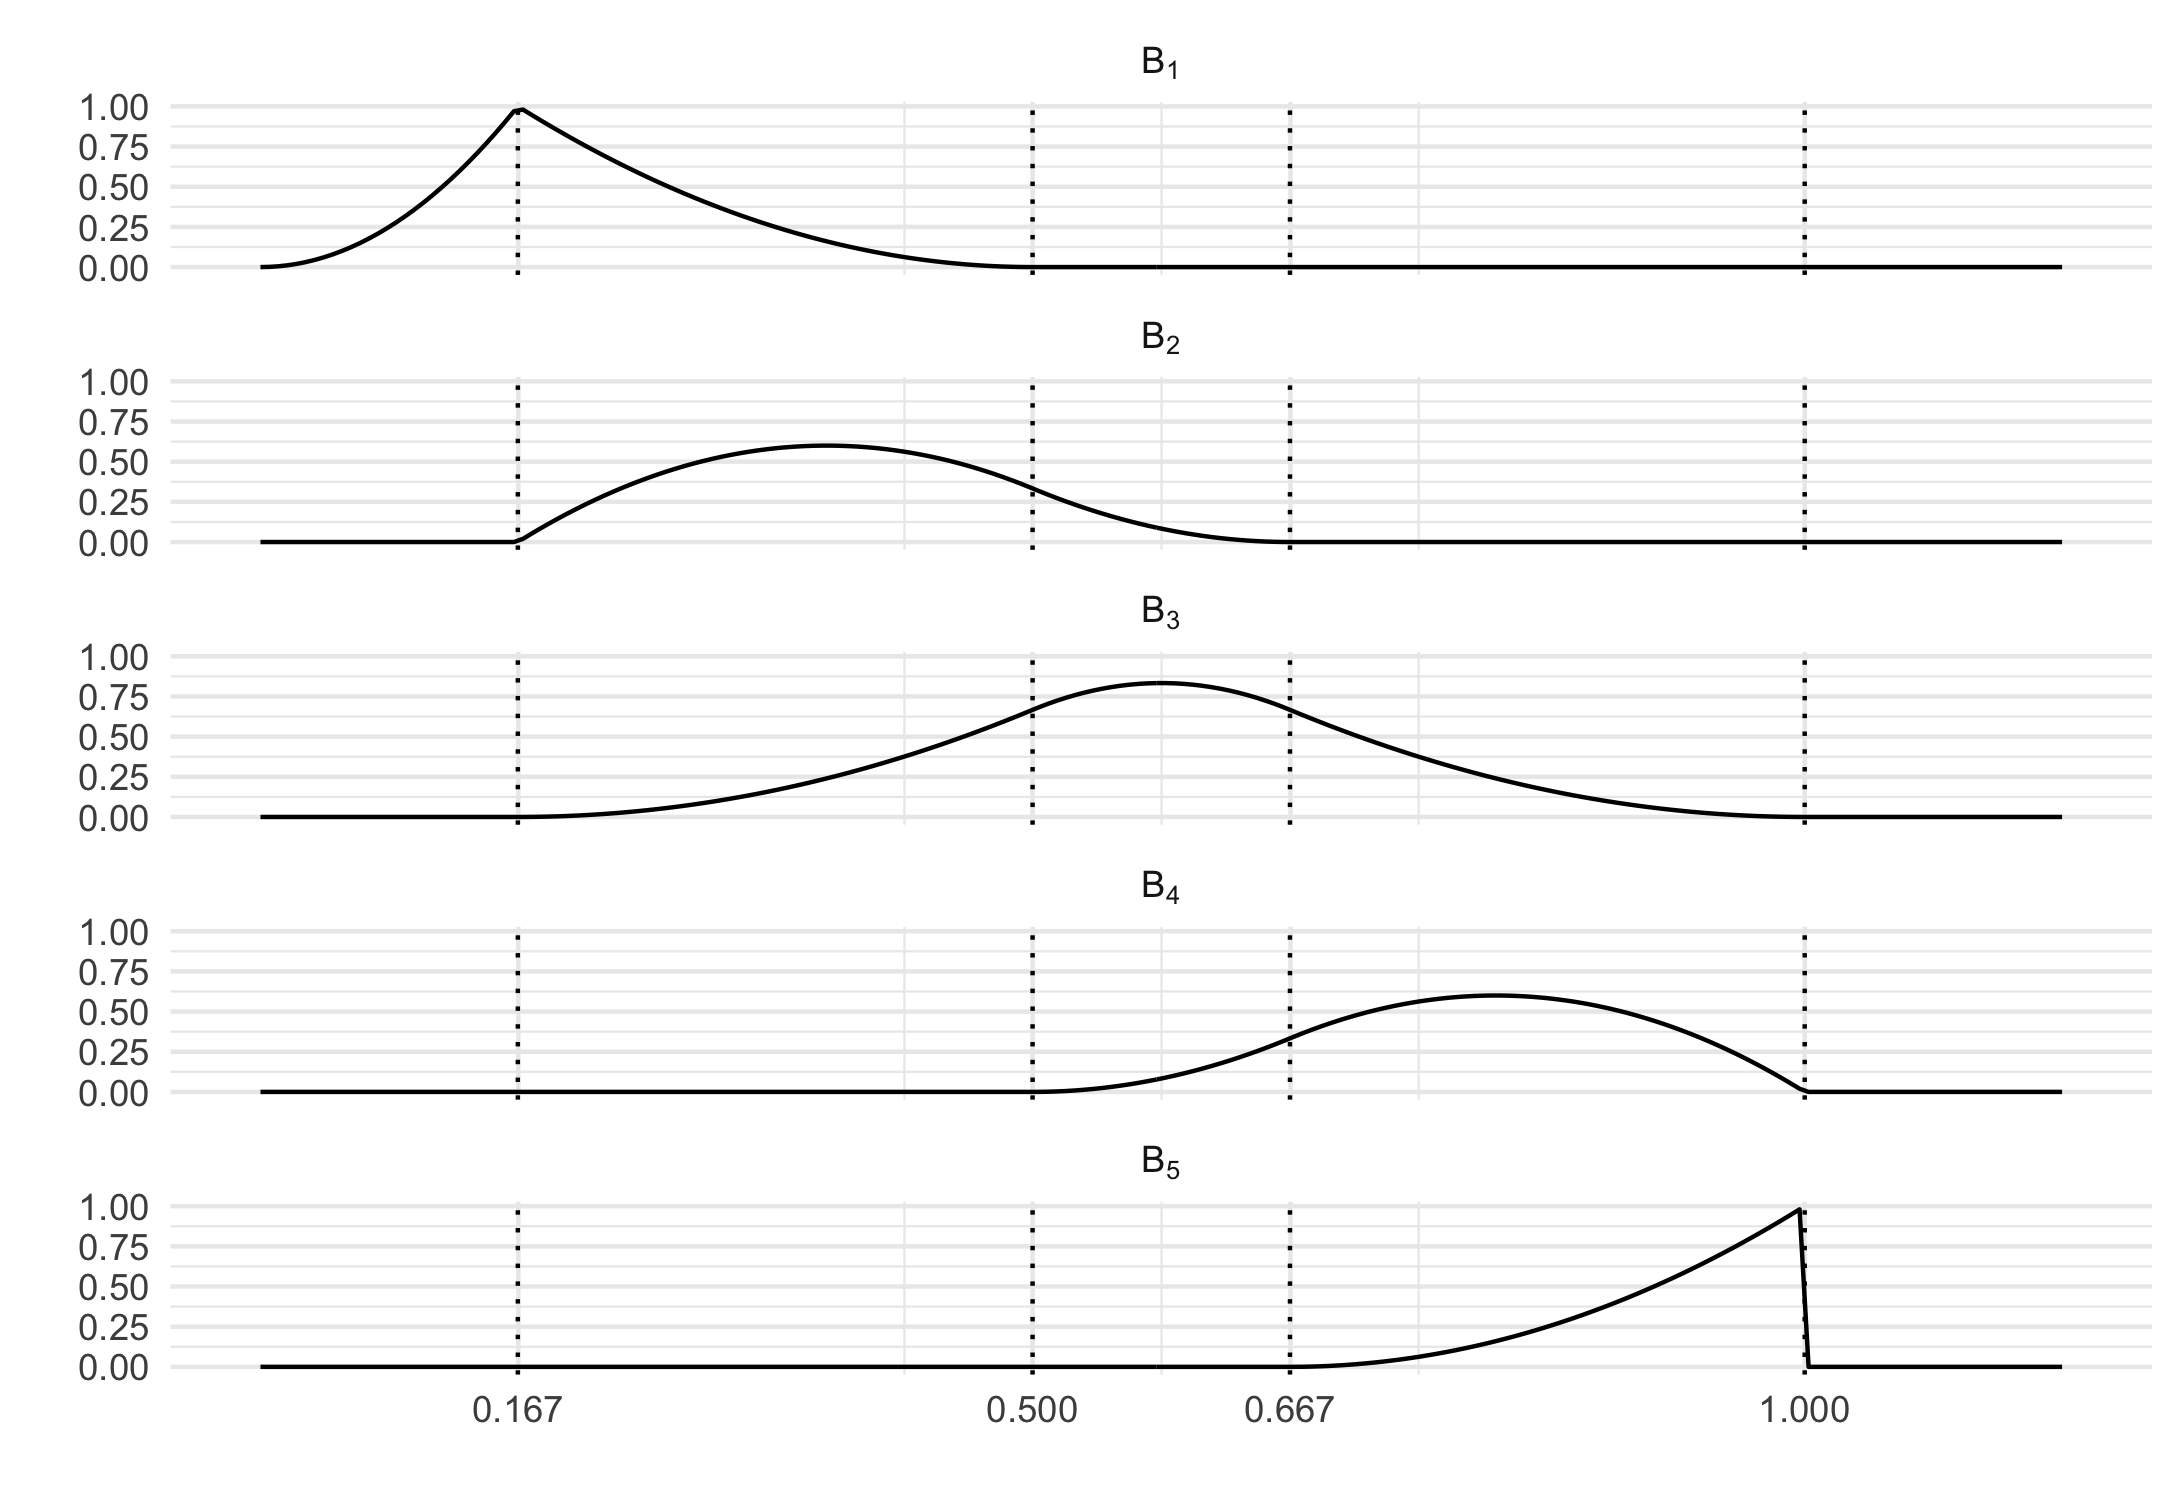
\includegraphics{deboor_parabolic_bsplines.png}
%  %\caption{Parabolic B-splines corresponding to knot sequence $\{0,1,1,3,4,6,6,6\}$, illustrating the connection between knot multiplicity and smoothness.}\label{fig:deboor_bspline_basis}
%\end{center}
%\end{figure}
%\end{example}


\begin{definition} \label{B_representation_definition}
The \emph{B-representation of } $f \in \PP_{k,\xi,\nu}$ consists of 
\begin{enumerate}
\item \label{eq:first_B_rep_piece} integers $k$ and $n$ specifying the order of $f$ as a pp function and the number of linear parameters, 
\[
n = kl - \sum_{i}\nu_i = \mbox{dim}\left(\PP_{k,\xi,\nu}\right),
\]
respectively. 
\item \label{eq:second_B_rep_piece}The knot vector $t = \left \{t_i \right\}$, $i=1,\dots, n+k$ with elements arranged in increasing order, constructed according to Theorem~\ref{curryschoenbergthm}, via $\xi$ and $\nu$.
\item \label{eq:third_B_rep_piece} The B-spline coefficients $\alpha=\left \{\alpha_i \right\}$, $i=1 ,\dots, n$ for the knot sequence, $t$.
\end{enumerate}
\end{definition}
\vspace{1pt}
Given \ref{eq:first_B_rep_piece}, \ref{eq:second_B_rep_piece}, and \ref{eq:third_B_rep_piece} in \ref{B_representation_definition}, the function value at $x\in \left[t_k, t_{n+1}\right]$ is given by 
\begin{equation*}
f\left(x\right) = \sum_{i=1}^n \alpha_i B_i\left(x\right),
\end{equation*}
and in particular, by \ref{eq:BS_property_1}, for $x\in \left[t_j, t_{j+1} \right]$,
\[
f\left(x\right) = \sum_{i=j}^{j+k-1} \alpha_i B_i\left(x\right).
\]


